\documentclass[8pt, A4]{article}

%Margenes de la pagina.  otra opcion, usar \usepackage{a4wide}
\usepackage[paper=a4paper, left=1.7cm, right=1.7cm, bottom=1.7cm, top=1.7cm]{geometry}
\usepackage{color}

%este paquete permite incluir acentos.  Notar que espera un formato ANSI-blah de archivo.  Si en lugar de eso se tiene un utf8 (usual en los linux), entonces usar \usepackage[utf8]{inputenc}
\usepackage[utf8]{inputenc}

%Este paquete es para que algunos titulos (como Tabla de Contenidos) esten en castellano
\usepackage[spanish]{babel}

%El siguiente paquete permite escribir la caratula facilmente
\usepackage{caratula}

\usepackage{verbatim}

\usepackage{aed2-symb,aed2-itef,aed2-tad,aed2-tokenizer,modulos_diseno, ./algorithms/clrscode3e}
\usepackage{framed}
\usepackage{amsmath}

\usepackage{graphicx}

%Datos para la caratula
\materia{Algoritmos y Estructuras de Datos III}

\titulo{Trabajo Pr\'actico 3}


\integrante{Ortiz de Zarate, Juan Manuel}{403/10}{jmanuoz@gmail.com}
\integrante{Martelletti, Pablo}{849/11}{pmartelletti@gmail.com}
\integrante{Kujawski, Kevin}{459/10}{kevinkuja@gmail.com}
\integrante{Carreiro, Martin}{45/10}{carreiromartin@gmail.com}

\begin{document}
%numero de grupo
{\hfill\Huge 10}
%esto construye la caractula
\maketitle 

 
 \tableofcontents

 \newpage

%\section{Introducci\'on}
En el siguiente trabajo presentaremos la resolución a tres problemas que se nos dio a resolver. Mostraremos para cada uno
el algoritmo que utilizamos para resolverlo describiendo que técnicas de las vistas en clase utilizamos, mostraremos también
el análisis de complejidad de cada algoritmo y mostraremos gráficamente los resultados de las mediciones para ver si se cumple el análisis 
teórico.


% \newpage
\section{Problema 1}

\subsection{Enunciado}
El enunciado nos plantea una situación en donde tenemos un edificio con n pisos y personas en cada piso que quiere ir a planta baja. Para poder hacerlo, el edificio provee un 
ascensor que deberá buscar a las personas para poder bajarlas. 
Este ascensor posee energía y capacidad limitada que no le permite recorrer siempre todos los pisos y levantar todas las personas, por lo tanto queremos maximizar la cantidad
de personas a descender del edificio dado la cantidad de personas por piso, su energía y la capacidad.

\subsection{Soluci\'on}
La solución planteada utiliza Programación Dinámica a través de decisiones. Es decir, planteamos el problema de forma tal que en vez de maximizar la cantidad de personas que 
pueden descender, encontramos el máximo valor posible que va a estar ubicado entre cero y la cantidad de personas total en el edificio.\\
A continuación se explicará cómo se resolvió el problema:\\
Primero obtenemos la cantidad total de personas recorriendo el edificio dado, y buscaremos ese dicho máximo valor.
Para ello, utilizaremos la conocida búsqueda binaria en la cantidad de personas en el edificio, hasta encontrar el valor tal que el siguiente no sea posible levantarlo y sin embargo el número que estoy evaluando si.
Por lo tanto lo único que resta, es ver si se puede levantar esa cantidad de personas dada la capacidad del ascensor, su energía y un edificio. \\
Para poder levantar esas personas buscaremos el piso mínimo al que necesitamos ir para poder levantar la cantidad de personas requeridas$^*$. Recorreremos el edificio desde ese piso mínimo hacia abajo, en caso de
ser posible llegar hasta él y poder volver a descender, levantando la máxima cantidad de personas de cada piso en el camino hasta llenar la capacidad. Una vez completada, descenderemos a los pasajeros y volveremos a repetir el proceso
para el mismo piso en caso de que haya quedado gente, o el siguiente en caso de haberlo vaciado o no poder llegar por poca energía, hasta que levantemos la cantidad requerida (caso que devolveremos que se puede) o hasta que nos quedemos sin energía (caso que devolveremos que no se puede). Tener en cuenta que el piso elegido como mínimo puede contener más cantidad de gente que la requerida por lo tanto puede pasar que no levantemos gente y que sin embargo, descendamos la cantidad requeridad personas.\\
Para la demostración de la resolución, explicaremos por qué el piso elegido previamente es el correcto, y por qué la estrategia de levantar de arriba hacia abajo es verdadera.
Este piso mínimo es la mejor opción ya que si subimos más pisos estaríamos utilizando energía para levantar la misma cantidad de gente que podríamos encontrar en los pisos
inferiores, y no se puede ir más abajo porque si no, tenemos la cantidad de gente necesaria para poder levantar el valor pedido.\\
Definimos el mundo de las estrategias, como el conjunto de estrategias posibles y definimos estrategia como el método por el que se levanta gente. Cómo no nos interesa
la energía utilizada, ya que solo queremos ver si puede levantar la cantidad de personas mencionada, y no la optimalidad de energía, una estrategia estará conformada por el
conjunto de personas que levanta en cada piso. De este mundo de estrategias, tomaremos solo aquellas que su piso más alto en el cual levantan personas es el nuestro, y que
levanten la misma cantidad que nosotros. Este conjunto es distinto de vacío ya que es un conjunto acotado de personas y pisos, por lo tanto se van a poder levantar a partir de
cierta energía dada. Ahora queremos ver que nuestra estrategia se encuentra en este conjunto. Para ello, tomaremos una de esas estrategias E y veremos que se puede permutar de tal
forma que consigamos nuestra estrategia. Esta permutación se debe a que si la estrategia E 


\small {\textbf{*} Para ubicar este piso mínimo recorreremos el edificio desde abajo contando la cantida de personas en los pisos, hasta que el valor sea mayor o igual al requerido.}




\subsection{Pseudoc\'odigo}
\begin{codebox}
\Procname{$\proc{resolver}$ (\textbf{in} $capacidad$, \textbf{in} $energia$, \textbf{in} $pisos$)}{maximaCantidad}{Int}
\li		totalPersonas = SumaTotalPersonas(pisos);
\li		return BusquedaBinariaPersonas(0,totalPersonas, totalPersonas,energia,capacidad,pisos);
\end{codebox}

\begin{codebox}
\Procname{$\proc{SumaTotalPersonas}$ (\textbf{in} $pisos$)}{acum}{Int}
\li		\textbf{Para} cada piso p \Do
\li			acum = acum + genteEnPiso(p) \End
\end{codebox}

\begin{codebox}
\Procname{$\proc{BusquedaBinariaPersonas}$ (\textbf{in} $desde$, \textbf{in} $hasta$, \textbf{in} $total$,\textbf{in} $energia$, \textbf{in} $capacidad$, \textbf{in} $pisos$)}{acum}{Int}
\li		medio = (desde + hasta)/2;
\li		puedo = sePuedeLevantar(energia, capacidad, pisos, medio);
\li 		\textbf{Si} puedo \Do
\li				\textbf{Si} no se puede levantar el siguiente terminé
\li 				\textbf{Si no} busquedaBinariaPersonas en la siguiente mitad \End
\li 		\textbf{Si no} busquedaBinariaPersonas en la primera mitad
\end{codebox}

\begin{codebox}
\Procname{$\proc{sePuedeLevantar}$ (\textbf{in} $energia$, \textbf{in} $capacidad$, \textbf{in} $pisos$, \textbf{in} $personasABuscar$)}{sePuede}{Boolean}
\li 		\textbf{Para} cada piso empezando desde el piso minimo \Do
\li			\textbf{Si} tengoEnergiaParaLlegar y Hay Gente \Do
\li				\textbf{Si} el piso tiene mas gente que mi capacidad \Do
\li					sumoLoQueLevante
\li					veoSiPuedoVolverAEstePiso \End
\li				\textbf{Si no} \Do
\li					sumoLoQueLevante
\li					mientrasBajoSumoGenteParandoEnLosPisosQueHayGente \End \End
\li			\textbf{Si no} \Do
\li				AnotoLasQueNoLevanté \End \End
\li		return (cuantoLevante >= personasABuscar)
\end{codebox}


\subsection{Analisís de complejidad}	
Para averiguar cuanta gente hay en todo el edificio tenemos que recorrer todo el vector 'pisos' e ir sumando la cantidad de gente en cada piso. Eso nos cuesto O(n) donde n es la cantidad de pisos. Luego hacemos una búsqueda binaria sobre la cantidad total de gente que mediante la función sePuedeLevantar busca el máximo de gente que es posible cargar. La complejidad de la búsqueda binaria es de O(log cantGente) (esto es sabido, porque ya lo vimos en algoritmos y estructura de datos 2) y la complejidad de la función sePuedeLevantar en el peor caso (sería cuando tiene que irse hasta el último piso para poder levantar la cantidad de gente solicitada y tiene energía suficiente para levantarlos a todos) es de: \\
	O( $\sum\limits_{i=0}^{n} { ( \lceil (pisos[i]/capacidad) \rceil  + i}$ ) ) \\
Esto es porque por cada piso al que voy tengo que ir tantas veces tal que levante el total de gente de ese piso (eso es $\lceil$pisos[i]/capacidad$\rceil$) y luego en caso que me haya sobrado espacio voy recorriendo todos los pisos inferiores para llenar la capacidad restante.
Finalmente la complejidad total del ejercicio nos queda:\\
O( n + Log(g) * $\sum\limits_{i=0}^{n} { ( \lceil (pisos[i]/capacidad) \rceil  + i ) }$ ) \\
Donde n es la cantidad total de pisos y g la cantidad total de gente en todo el edificio.

\subsection{Tests y Gráficos}
Con respecto a los tests realizados, los mismos no se hicieron en cuanto a la complejidad (ya que al utilizar estructuras primitivas de java, podemos asegurar que la complejidad de cada una de sus operaciones es la que aparece en la documentación de ellas y por tanto, es la que detallamos en el apartado anterior), sino en cuanto a la cantidad de ciclos que realiza cada solución (más precisamente, la creación del árbol generador mínimo) para distintas instancias, de acuerdo a la cantidad de vértices (localidades) y aristas (enlaces) que posee cada una.
Como podemos apreciar en los siguientes gráficos, la cantidad de ciclos, para grafos en donde la cantidad de aristas es la misma, es directamente proporcional a la cantidad de vértices que contenga el mismo (figura 1). Es cierto que en algunos casos ésto no se cumple pero, en el caso promedio, a más cantidad de vértices, con igual cantidad de aristas, más ciclos tendrá que hacer nuestro algoritmo para encontrar el AGM válido. Los casos extremos serían aquellos en donde las aristas se insertan ordenados de la misma forma que los leerá nuestro algoritmo, donde la cantidad de ciclos se corresponde con la cantidad de vértices. Por el contrario, el peor caso se da cuando hay muchas aristas de 2 vértices que ya fueron visitados, de menor peso de aquellas que contengan 1 vértice visitado y otro sin visitar. De ésta forma, el algoritmo hará tantos ciclos como aristas tenga el vértice para, recién en la último, procesar el vértice y agregarlo al AGM.
\begin {center}
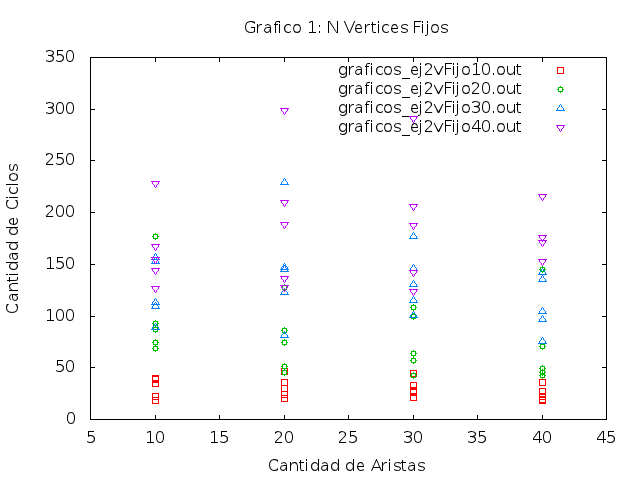
\includegraphics[width=8cm]{./graficos/grafico_vfijo.png}
% grafico.eps: 0x0 pixel, 300dpi, 0.00x0.00 cm, bb=50 50 410 302
\end {center} 
Por otro lado, y con respecto a la figura 2, donde la cantidad de aristas está fijo, vemos que la cantidad de ciclos que se llevan a cabo es netamente aleatorio, ya que, de acuerdo a cómo estén distribuidas las distintas aristas y sus pesos, es posible crear el AGM en n pasos, siendo n la cantida de vértices, o bien, en n x e(n), siendo e(n) la cantidad de aristas de n. El primer caso se daría sólo cuando el grafo que analizamos posee aristas minimas sin descubrir en todos los pasos, mientras que el peor caso, que sería el de recorrer todas las aristas del vértice, es el mismo que analizamos en el párrafo anterior.
\begin {center}
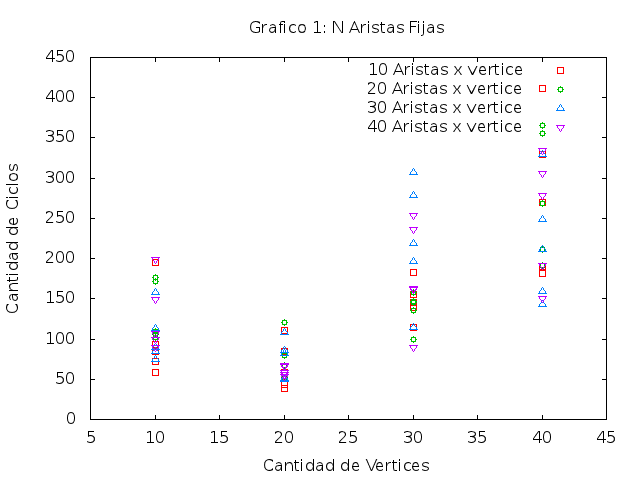
\includegraphics[width=8cm]{./graficos/grafico_efijo.png}
% grafico.eps: 0x0 pixel, 300dpi, 0.00x0.00 cm, bb=50 50 410 302
\end {center} 


\subsection{Conclusiones}
El problema nos mostró que podía ser encarado de distintas maneras dentro de la métodología de programación dinámica. Al principio habíamos utilizado una idea parecida a la de SubSetSum con memorization pero no podíamos hacer funcionar el algoritmo. Sin embargo, encaramos el problema a través de decisiones lo que nos ayudó a entender el principio de ptimalidad.

  \newpage
\section{Problema 2}

\subsection{Enunciado}
En este ejercicio se nos solicita buscar el conjunto dominante mínimo y óptimo dado un grafo cualquiera. Este es un problema del tipo NP completo 
para el cual aún no se encontró forma de resolverlo polinomialmente pero tampoco se demostró que no sea posible solucionarlo con dicha complejidad.

\subsection{Soluci\'on}
Como todavía no se halló algoritmo alguno para resolverlo poliniomalmente y nosotros no somos investigadores/iluminados (aún) decidimos resolverlo
de manera exponencial. Para esto utilizamos el popular método (dicho en criollo) de quedarme con la mejor opción entre poner y no un nodo en el 
conjunto dominante. Este procedimiento lo que hace, básicamente, es analizar todas las soluciones posibles y agarrar la mejor de ellas. 
No nos pareció primordial agregarle memorization ya que su complejidad no mejoriría de forma considerable y tampoco nos pareció imperante 
preocuparnos por la complejidad de la función que chequea si el conjunto recibido es dominante, ya que, mientras sea polinimal, va ser despreciable 
al lado de la complejidad de analizar todas las soluciones (que como dijimos es exponencial).

\subsection{Pseudocódigo}

global grafoOriginal

\begin{codebox}
\Procname{$\proc{obtenerConjuntoDominanteMinimo}$ (\textbf{in} $Grafo$)}{mesetaMaxima}{Int}
\li	c = crearConj()
\li	grafoOriginal = Grafo
\li	return buscarMinimo(Grafo,c)
\end{codebox}

buscarMinimo(grafo, conjuntoDom){
	if(esDominante(conjuntoDom)){
		return conjuntoDom
	}else{
		vertice = grafo.obtenerVertice(); 
		grafo = grafo.sinUno()
		return min(buscarMinimo(grafo, conjuntoDom), buscarMinimo(grafo, conjuntoDom + vertice)
	}
}

esDominante(grafo, conjuntoDom){
	foreach(v en V(grafoOriginal)){
		if(conjuntoDom.esta?(v){
			continue
		}else{
			encontre = false
			foreach(ver en conjuntoDOm){
				if(ver.adyacentes.esta?(v))
					break
			}
			if(!encontre)
				return false
		}
	}
	return true
}

La complejidad de mi algoritmo es de 2^n * n³. Voy a demostrarlo por inducción:

Caso Base:

n = 1, si n tiene un solo nodo ver si es dominante me cuesta O(1) ya que recorrer los vertices del grafo original es una sola iteracion y no es posible recorrer sus aristas. Luego divido en el caso en el que uso a ese nodo en el conjunto dominante y el caso en que no. El caso en que no al no tener mas nodos con cual probar me va a devolver el grafo original y el otro caso también ya que el grafo original era el que contenía únicamente a ese nodo. Ambos casos ver si el conjunto es dominante cuesta O(1) ya que tiene a lo sumo una iteración para hacer. Por lo tanto el algoritmo costaría O(1) que es igual a O(2¹*1³).

Hipótesis inductiva:

Supongo que con n nodos la complejidad es 2^n * n³

Paso inductivo:

Quiero ver que con n+1 nodos la complejidad pertenece a 2^(n+1)*(n+1)³

Ver si el conjunto vacío es dominante me cuesta O(1) ya que en la primera iteración del grafoOriginal no es posible encontrar ningún vertice en el conjunto dominante o adyacente a él. Luego obtengo un nodo del grafo (grafo en el que me guarde todos los vertices, no el origianl) y busco el minimo conjunto dominante agregando ese nodo al conjunto o no, esto por hipótesis inductiva me cuesta 2 * (2^n * n³), ya que tengo que calcular 2 veces el conjunto minimo para n nodos. Por lo tanto la complejidad me termina costando  2^(n+1)*n³ y esto pertence a 2^(n+1)*(n+1)³. Con lo cual queda demostrada la complejidad.

Notar que esta complejidad esta por encima de la complejidad exacta, ya que el n³ variaría en cada iteración dependiendo de la cantidad de nodos en el conjuntoDominante.


\subsection{Peor Caso}

Como el algoritmo es exacto y recorre todas las soluciones posibles siempre obtiene la mejor de ellas. Por lo tanto no existe una 'peor' instancia
en la que la solución devuelta sea sub-óptima, siempre devuelve la mejor.

\subsection{Tests y análisis}




  \newpage
\section{Algoritmo Goloso}

\subsection{Soluci\'on}

Proponemos una solución heuristica golosa para encontrar un conjunto dominante de un grafo lo mas pequeño posible con una complejidad polinomial.\\
Para ello nos basamos en una estrategia de selección de nodos dominantes, la cual consiste en elegir el nodo que mas adyacentes no cubiertas tenga (es decir, que todavía no fueron dominadas) y verificando en cada iteración si el conjunto actual es dominante. En base a diferentes estrategias y tipos de grafos (estrella, bipartitos, completos, estrellas unidas, caminos, ciclos) que fuimos observando, elegimos esta ya que fue la que más nos convenció y mejores resultados nos dió debido a que siempre intenta seleccionar el nodo que mas pueda dominar a otros nodos reduciendo el conjunto de los no cubiertos y acercandose a una mejor solución del problema. 

\subsection{Pseudocódigo}

\begin{codebox}
\Procname{$\proc{MCDGreedy}$ (\textbf{in} $Grafo$)}{conjuntoDomGoloso}{ConjDeVértices}
\li	vértices = lista de vértices del grafo	\RComment O(n)
\li	dominantes = conjunto vacio de vértices	
\li	\textbf{Mientras} no estén TodasCubiertas(vértices) \Do \RComment O($n^3$)
\li 		Ordeno los vértices por la cantidad adyacentes que tenga no cubiertas (sin dominar), de mayor a menor. \RComment O(n*log(n))
\li 		Elijo como dominante al primero de la lista y lo agrego al conjunto de \textbf{dominantes} \RComment O(n)
\li 		Saco de la lista de vértices al elegido \RComment O(n)
\li 		ActualizarGradoSinDominar(elegido) \RComment Actualizo los nodos del grafo,\\ disminuyendo la cantidad de \textit{grado sin dominar} de los adyacentes al elegido, y de los adyacentes a estos.  O($n^2$)
\End
\li	\textbf{return} dominantes
\end{codebox}

\begin{codebox}
\Procname{$\proc{TodasCubiertas}$ (\textbf{in} $ListaDeVertices$)}{result}{Boolean}
\li 	\textbf{Mientras} haya vértices en la lista \Do
\li 		\textbf{Si} el vértice no esta dominado \Do
\li 			\textbf{return} falso \End \End
\li 	\textbf{return} verdadero
\end{codebox}

\begin{codebox}
\Procname{$\proc{ActualizarGradoSinDominar}$ (\textbf{in} $Vertice elegido$)}{}{}
\li 	Marcar al vértice elegido como dominado.
\li 	unionDeAdyacentes = lista de vértices vacia, que luego se usará para actualizar.
\li 	\textbf{Mientras} haya vértices en la lista de adyacentes al \textbf{elegido} \Do
\li 		\textbf{Si} el vértice \textit{elegido} no estaba dominado \Do
\li 			Decremento en uno el grado de adyacentes sin dominar del nodo actual \End
\li 		\textbf{Si} el nodo actual \textit{elegido} no estaba dominado \Do
\li 			Agrego los nodos adyacentes a la lista \textit{unionDeAdyacentes} \End
\li 		Marco al nodo actual como dominado. \End
\li 	\textbf{Mientras} haya vértices en la lista unionDeAdyacentes \Do 
\li 			Decremento en uno el grado de adyacentes sin dominar del nodo actual \End %\RComment Recorro unionDeAdyacentes para actualizar\\  el grado de nodos adyacentes sin dominar
\end{codebox}

\section{Análisis de Complejidad}

La complejidad del algoritmo es de O($n^3$)

El algoritmo comienza creando una lista de vértices en O(n).\\
Luego entra en un ciclo que como máximo será lineal en la cantidad de vértices. En cada iteración deberá comprobar si el conjunto actual de vértices elegidos domina todo el grafo O($n^2$), ordenar todos los vértices O(n*log(n)), elegir un vértice O(1), removerlo de la lista O(n) y finalmente actualizar el atributo de los grados sin dominar adyacentes de cada nodo O($n^2$), esto es porque para los adyacentes del nodo elegido y a su vez para los adyacentes de estos tengo que bajar en uno este atributo, recorrer los adyacentes me lleva O(n) y por cada adyacente recorrer sus adyacentes también me lleva O(n), O(n) * O(n) = O($n^2$).\\

Por lo tanto, la complejidad nos queda:\\
O(n) + O(n) * (O($n^2$) + O(n*log(n) + O(n) + O($n^2$)) = O($n^3$)\\\\

La complejidad final del algoritmo goloso es de O($n^3$), cumpliendo el objetivo de ser polinomial.


\subsection{Peor Caso}

Al ser una heurística, en cierto casos la solución no es la optima que podría dar un algoritmo exacto, pero aún asi es correcta.
Los peores casos, donde se produce una diferencia en el tamaño de conjunto dominante respecto a la optima, se suelen dar en grafos en los que varios nodos tienen el mismo grado o hay pequeña diferencia, y esto es debido que para la elección del vertice dominante en cada iteración nos quedamos con el que mayor grado de nodos adyacentes no cubiertos tenga y si hay varios con esta misma característica puede pasar que el nodo seleccionado no sea conveniente a futuro para llegar a una solución optima.

En los siguientes ejemplos de grafos se puede apreciar mejor:

\begin {center}
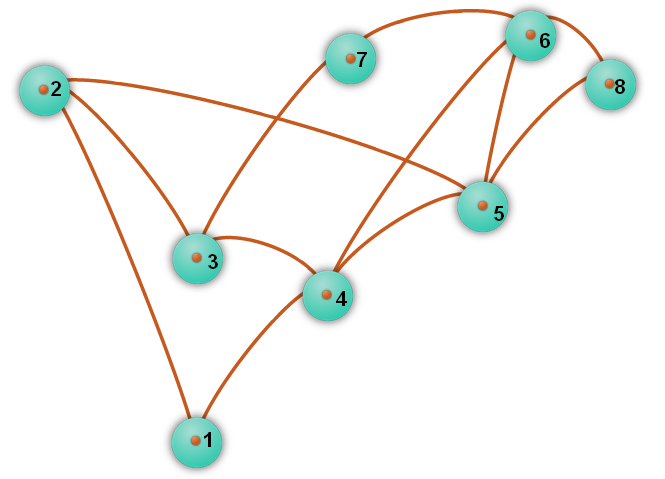
\includegraphics[width=8cm]{./graficos/grafo.png}
% grafico.eps: 0x0 pixel, 300dpi, 0.00x0.00 cm, bb=50 50 410 302
\end {center} 
La solución optima proporcionada por el algoritmo exacto es {6,2}, mientras que el goloso devuelve {4,3,5}, ya que como los nodos 6,4 y 5 tienen el mismo grado, al momento de la elección se decide por el 4 provocando esta diferencia en el tamaño del conjunto con respecto a la solución optima.

\begin {center}
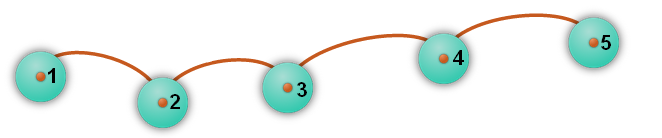
\includegraphics[width=8cm]{./graficos/grafo_camino.png}
% grafico.eps: 0x0 pixel, 300dpi, 0.00x0.00 cm, bb=50 50 410 302
\end {center} 
La solución óptima proporcionada por el algoritmo exacto es {2,4}, mientras que el goloso podría devolver {3,2,5}, ya que como los nodos 2, 3 y 4 tienen el mismo grado, si se decide por el 3, dejaría a todos los demas nodos con 1 grado sin dominar y faltando los dos extremos, provocando que si o si se necesite cubrirlos o elegirlos como dominantes, haciendo que el conjunto tenga tamaño 3 y no 2 como el exacto.

\subsection{Tests y análisis}

En los gráficos que aparece a continuación  se puede notar que a medida que la cantidad de nodos aumenta, el algoritmo dibuja un comportamiento que se asemeja a O($n^3$) en relación a la cantidad de ciclos y el tiempo en nanosegundos.\\

\begin {center}
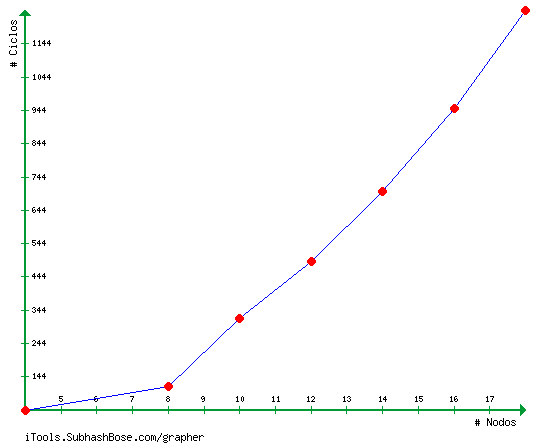
\includegraphics[width=8cm]{./graficos/goloso_1.png}
% grafico.eps: 0x0 pixel, 300dpi, 0.00x0.00 cm, bb=50 50 410 302
\end {center} 

\begin {center}
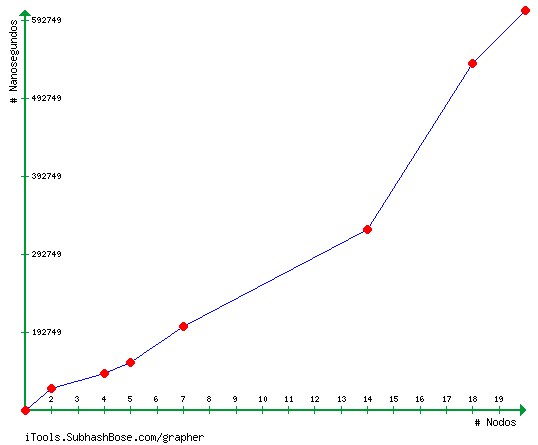
\includegraphics[width=8cm]{./graficos/goloso_2.png}
% grafico.eps: 0x0 pixel, 300dpi, 0.00x0.00 cm, bb=50 50 410 302
\end {center}

  \newpage
\section{Algoritmo Local Search}

\subsection{Solución}
La idea de un algorítmo de búsqueda local (o local search) es, a partir de una solución (no óptima) a un problema dado, trabajar sobre ella, realizar distintas operaciones y estrategias de modo tal de mejorarla e intentar acercarse lo más posible a una solución óptima. La dinstinción de éstos algoritmos está en que cada modificación a la solución original, nos genera una o un conjunto de soluciones al problema, siempre "cercanas" a la solución que fue modificada. \\
En nuestro caso en particular, la idea es que, a partir de un grafo, hallemos un cojunto dominante de alguna forma (todos los nodos del grafo son, en efecto, un cojunto dominante. O bien también podemos usar la solución obtenida con el algortimo greedy) y, a partir de ella, intentemos construir, mediante estrategia y funciones creadas por nostros, a una nueva solución, mejor o igual a la que nos proveyeron como base. \\
Es así que nos planteamos lo siguiente: ¿qué operaciones podemos realizar de forma tal que, a partir de un conjunto dominate, no necesariamente mínimo, de forma tal de reduicir la cardinalidad del conjunto y que continúe siendo dominante? Las posibilidades que encontramos fueron orientadas siempre a la posibilidad de reducir o, al menos mantener, la cantidad de nodos en el conjunto dominante. Es por eso que las estrategias que utilizamos en la búsqueda local son las siguientes: 

\begin{description}
\item[Reemplazar 2 nodos del Conjunto] dominante por uno que se encuentre dominado. Ésta es la forma más directa de reducir la cardinalidad del CD. La forma de seleccionar los nodos intercambiables la realizamos verificando si la unión de nodos vecinos de los dos nodos a quitar del conjunto está incluida en el conjunto formado por los vecinos del vértice a insertar en el CD. Ésta es la forma más sencilla de encontrar dichos nodos, ya que de otra forma, el costo de encontrar estos posibles reemplazos sería muy costoso. Además, existe la posibilidad de encontrar varios posibles candidatos, por lo que ideamos 3 funciones de comparación para ordenar éstas tuplas y, en cada caso, utilizar la más "conveniente" según dicha función.
\item[Eliminar 1 nodo del CD:] Para éste caso, analizamos si elimiando alguno de los nodos del CD, el mismo sigue dominando a todos los nodos del grafo. Para ello, nos fijamos si el conjunto de vecinos del nodo que queremos quitar, está incluido en la unión de todos los vecinos de los nodos del CD menos el nodo que queremos quitar. Si es así, quitando el nodo el conjunto seguirá siendo dominante. En éste caso, es claro que la cardinalidad disminuye.
\item[Reemplar 1 nodo del CD] por otro del conjunto dominado. La estrategia aplicada para encontrar los posibles candidatos es la misma que en la técnica del 2x1, es decir, nos fijamos los nodos que estén en el CD, y buscamos aquellos dominados que tengan los mismos vecinos. Es claro que ésta técnica no reduce la cardinalidad del conjunto, pero la utilizamos con la esperanza de que éste cambio de nodos nos modifique la solución parcial y, a partir de ésta, si podamos utilzar algunas de las técnicas anteriores.
\end{description}

Si luego de k iteraciones, con $k$ aleatorio entre 10 y 20, el algoritmo no logra reducir la cardinalidad de la solución parcial, se decide que no será posible encontrar una solución cuya cardinalidad sea menor y, por tanto, se termina la ejecución, dando como solución al problema a la solución parcial, que tiene una cardinalidad igual o menor a la solución inicial dada al algortimo.

\subsection{Pseudocódigo}
\begin{codebox}
\Procname{$\proc{EncontrarSolucion}$ (\textbf{ConjuntoDominante} $cd$, \textbf{Comparator} $funcion$)}{cd}{Conjunto Dominante}
\li	elijo un k aleatorio entre 10 y 20.
\li	\textbf{hasta} que la cardinalidad de la solucion no cambie durante k estrategias: \Do
\li		ElegirEstrategia(cd, funcion)
\End
\End
\li	\textbf{return} cd
\end{codebox}

\begin{codebox}
\Procname{$\proc{ElegirEstrategia}$ (\textbf{ConjuntoDominante} $cd$, \textbf{Comparator} $f$)}{res}{Boolean}
\li	\textbf{para} cada una de las E estrategias: \Do
\li		intento la estregia E en el conjunto dominante cd
\li		\textbf{Si} es posible llevar a cabo la estrategia E con la funcion f: \Do
\li			devuelvo true
\End
\li		\textbf{Si} no es posible llevar a cabo la estrategia E, sigo con la proxima estrategia
\End
\li \textbf{si} no pude llevar a cabo ninguna estrategia, aumento el contador de estrategias fallidas
\li \textbf{return} false
\end{codebox}

\section{Análisis de Complejidad}
Para todos los casos, se corre al menos k veces, y para cada una de esas k corridas, se utilizan 3 métodos para intentar hallar una nueva solucion:
\begin{description}
\item[2x1:] Se crea una cola de nodos, ordenados por una funcion f (pasada por parametro). Para ello, se recorren todos los posibles pares de nodos dominantes, y para cada par, se analiza si es posible reemplazarlo por un nodo del conjunto dominado. La complejidad de crear esta cola es de $O(n^2)$, siempre y cuando se considere que $n^2$ es mayor a m, siendo m la cantidad de vertices del conjunto dominado. Luego, para hacer el intercambio, se realizan operaciones en ArrayList, que son $O(n)$. Por lo que la complejidad de éste método es de $O(n^2)$.
\item[QuitarUno:] en éste caso, se recorren todos los nodos del conjunto dominante, y se pregunta si, quitando el nodo en cuestion, el conjunto continúa siendo dominante. Ésta método tiene una complejidad de $O(n x m)$, donde n es la cantidad de nodos del cd, y m es la cantidad de aristas de cada nodo.
 \item[UnOxUnO] ésta estrategia requiere de recorrer todos los vértices dominantes, y para cada uno de ellos, compararlo con todos los vértices dominados, y fijarme si puedo intercambiar éstos nodos (en cuestión, si tienen los mismos vecinos) de forma tal que el conjunto continue siendo dominante. Esta verificación es de complejidad $O(n x m)$, donde n es la cantidad de nodos del conjunto dominante, y m la cantidad de nodos del conjunto dominado.
\end{description}
 
 Es decir, que la complejidad en todos los casos, no es mayor a $O(n^2)$, ya que en todos los casos se analiza primero la opción de hacer el 2x1. Si puede, la complejidad será esa, y si no puede, seguirá con los otros métodos que, a rasgos generales, nunca superan ésta cota de $O(n^2)$. Por lo que la complejidad general del algoritmo es de \textbf{$O(n^2)$}.
 
 \subsection{Peor Caso}
 Es claro que, al ser una heurística, en muchos casos la solución obtenida por la búsqueda local (o local search) no es la óptima, pero de todas formas, se trata de soluciones "cercanas" a ella. En éste sentido, se dan cuando los nodos de la solución de la cual se parte la búsqueda loca, tienen muchas aristas conectadas entre si o a otros vértices ya dominados (los grados de los nodos son muy altos). Ésto hace que, por ejemplo, las estrategias elegidas no puedan intercambiar nodos, o quitar nodos de la solución de la que se parta y, sin embargo, en la práctica si exista una solución con menor cantidad de nodos. \\
En particular, hemos encontrado dos casos generales distintos: por un lado, aquellos en que el algorítmo de búsqueda local mejora la solución de la cual se parte pero, sin embargo, no llega a una solución óptima (calculada a partir del mismo grafo con el algoritmo exácto). Y por otro lado están aquellas instancias que, a partir de una solución, no pueden ser mejoradas por la búsqueda local, a pesar de haber una solución óptima y exacta con una menor cantidad de nodos. Éstos dos casos se pueden ver en los tests que hemos corrido en el jUnit, y que lamentablemente, no hemos podido correr para instancias de más de 25 nodos, ya que la solución exacta (que es de orden exponencial) no llega a terminarse y, por tanto, no podemos comparar los valores de la búsqueda local con los valores exactos. \\
\begin{center}
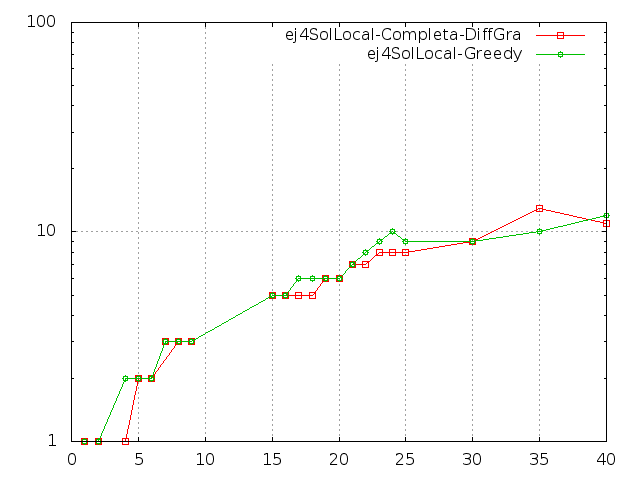
\includegraphics[width=12cm]{./graficos/comparacionSolucionPasadaLocal.png}
\end{center}
Éstos resultados, eran de esperarse, ya que se trata de una heurísitca y sólo en algunos casos partículares se consiguen los mismos resultados que en los algoritmos exáctos. La idea, entonces, es intentar de construir las mejores estrategias para poder llegar a un resultado lo más exacto posible, para instancias en que sea imposible (al menos hoy en día) correr el algoritmo exácto de orden exponencial. En éste caso particular, de la búsqueda local, seguramente haya muchas estrategias para mejorar o agregar, que nos aproximen a una solución un poco más exacta de la que encontramos hasta ahora, pero no pudimos dar con ellas.


\subsection{Tests y análisis}
En primer lugar, hemos hecho test para encontrar cuál de todas las funciones encuentra los nodos óptimos para el intercambio de nodos 2x1. En la teoría, todas analizan factores distintos, pero en la práctica, al ser muy pocos los nodos que pudimos intercambiar, las distintas funciones no han aportados cambios significativos en la cardinalidad de las soluciones. A lo sumo, ésta han diferido en 1 nodo, no más, y la que ha resultado más efectiva ha sido la de encontrar la diferencia de grados entre la tupla a quitar y el nodo a insertar. Es por eso que ésta función ha sido la que utilizamos para las pruebas restantes. \\
Una vez establecida qué función deberíamos utilizar para el 2x1, nos abocamos a testear el método de búsqueda local de acuerdo a la cantidad de nodos del grafo y el tiempo que le consume encontrar una solución. Vale aclarar que no tomamos en consideración el tiempo que nos consume encontrar una solución para darle a la búsqueda loca, ya que consideramos que ello no es parte de nuestro algoritmo. De ésta forma, podemos ver que nuestro algoritmo se comporta de forma polinómica en función del tiempo, como lo analizamos en la sección de complejidad. Es decir, mientras mayor cantidad de nodos tenga la solución que nos proveen, y más relacionados estén entre sí dichos nodos (es decir, a través de aristas hacia nodos del mismo conjunto o del conjunto de los dominados), mayor tiempo requerirá calcular nuestra solución. Además, y de forma conjunta con éste crecimiento, aumenta la cantidad de operaciones requeridas por el algortimo para finalizar cada iteración $k$, incremento que se ve directamente relacionado con el aumento de la cardinalidad de conjunto dominante. Ésto puede verse en el gráfico 1, de forma tal que a mayor cantidad de nodos que le pasamos a nuestra solución, mayor será el tiempo que le toma resolverlo, debido a que debe realizar más operaciones.

\begin{center}
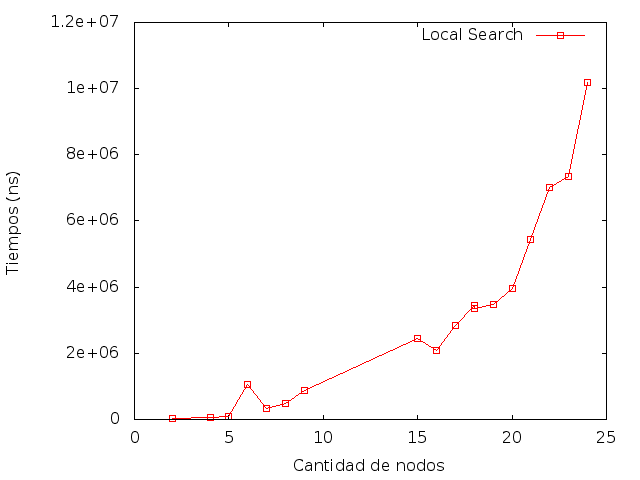
\includegraphics[width=13cm]{./graficos/tiempoLocalSearch.png}
\end{center}

Además, creemos conveniente probar / mostrar la mejoría que realiza nuestro algoritmo a las soluciones que se le dan. Para ello, comparamos la ejecución de la misma instancia para el algoritmo exacto, el algoritmo greedy y el algoritmo de solución local, y la calidad de la solución (la cardinalidad de las mismas), mostrando cómo mejoran las mismas de acuerdo a cada método. Es válido aclarar que en todas las corridas, hemos utilizado como instancia de entrada para el local search la solución  dada por el algoritmo greedy, por lo que en todos los casos, la cardinalidad de las soluciones de la búsqueda loca, será por lo menos, igual a la greedy y como máximo, si tuvimos suerte, igual a la exacta.

\begin{center}
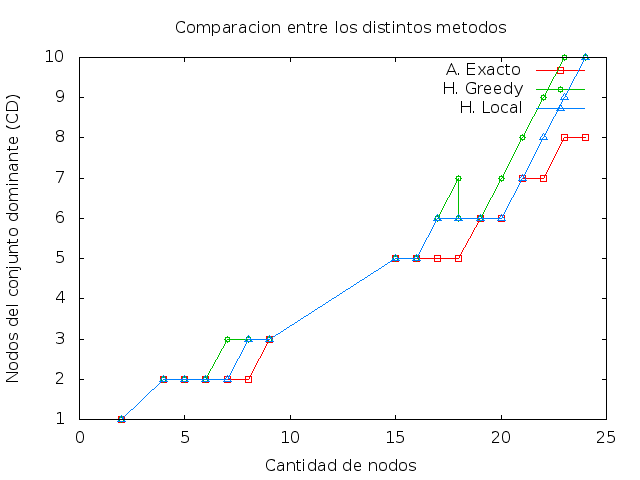
\includegraphics[width=13cm]{./graficos/local_comparacion_soluciones.png}
\end{center}

  \newpage
\section{Algoritmo GRASP}

\subsection{Solución}
La idea de este algoritmo es ejecutar una serie de veces nuestro algoritmo GREEDY randomizado y mejorarlo con la búsqueda local, guardando la mejor solución hasta el momento.
Esa randomización se debe a que el método por el cuál dicho algoritmo goloso elige siempre el mejor valor bajo su criterio, es ahora aleatorizada seleccionando al azar entre los primeros k elementos de la
lista de nodos a ser considerado dominante.\\
Para ello, agregamos en el algoritmo Greedy que reciba por parámetro dicho k, de forma tal que al momento de elegir el próximo nodo, en vez de elegir el primero de los nodos ordenados por la cantidad de adyacentes
sin dominar, ahora elige la posición i, que será el número obtenido pseudo-aleatoriamente a través de la función random entre 0 y k. En caso de que este k sea mayor a la cantidad de nodos considerados en la lista, 
k se definirá como la longitud de dicha lista.\\
Un tema importante de GRASP es que nunca termina, y neceista una condición de parada arbitraria. Elegimos, al igual que en LocalSearch, una iteración que busque hasta k veces asumiendo que
de las k*$|$MinConjDominante$|$ posibles soluciones que me puede devolver en cada iteración el algoritmo greedy.

\subsection{Pseudocódigo}

\begin{codebox}
\Procname{$\proc{MCDGrasp}$ (\textbf{in} $Grafo$, \textbf{in} $k$)}{ConjDominante}{Conj}
\li	mejorSolucion = TodosLosVertices
\li \textbf{Para} i=0 hasta k \Do
\li 	instanciaSolucionGreedyRandomized = MCDGreedy(grafo,k)
\li	nuevaSolucion = MCDLocalSearch(instanciaSolucionGreedyRandomized)
\li 	\textbf{Si} cantNodosDominantes(nuevaSolucion) $<$ cantNodosDominantes(mejorSolucion)  \Do
\li		mejorSolucion = nuevaSolucion
	\End
    \End	
\li	\textbf{return} mejorSolucion	
\end{codebox}
Se debe aclarar que tanto LocalSearch como Greedy devuelven ConjuntosDominantes verdaderos, por lo que lo único que importa es la cantidad de nodos devuelta.\\

A continuación se agrega el cambio hecho en el algoritmo greedy para aleatorizar la selección de nodos:\\
\begin{codebox}
\Procname{$\proc{elegirVertice}$ (\textbf{in} $ListaVerticesORdenada$, \textbf{in} $k$)}{proxVertice}{Vertice}	
\li     \textbf{Si} k $>$ $|$ListaVerticesORdenada$|$ \Do
\li 		k = $|$ListaVerticesORdenada$|$;
\End
\li 	posiciónAElegir = random(0,k);
\li	proxVertice = ListaVerticesORdenada[posiciónAElegir]
\li 	\textbf{return} proxVertice
\end{codebox}

\subsection{Análisis de Complejidad}
Por la demostración de la complejidad de la búsqueda local, sabemos que la complejidad es: O($n^2$);\\
Por la demostración de la complejidad del goloso, sabemos que la complejidad es: O($n^3$);\\
Dentro del GRASP se realizan k iteraciones de las siguientes operaciones:
\begin{itemize}
\item Ejecutar algoritmo goloso con random
\item Ejecutar algoritmo localSearch a partir de la solución del goloso
\item Comparar mejorSolución con nuevaSolución (esta operación es en O(1) ya que tanto conseguir el tamaño de un ArrayList en Java como la comparación de enteros es en O(1)) 
\end{itemize}
Esto es O(k*(goloso + localSearch)), que resulta polinomial.\\
Entonces la complejidad resulta O(k*$n^3$);

\subsection{Peor Caso}
Antes de hacer el gráfico, deberíamos calcular cual es el peor caso para este algoritmo. Sin embargo, el mismo depende de dos cosas:
\begin{itemize}
\item La solución random generada por el algoritmo goloso cuando se usa el valor de k. 	Esto es importante, ya que mientras esa solución sea generada de forma pseudo-random, menor cantidad
	de operaciones va a haber en la búsqueda local.
\item No se pudo determinar un peor caso para la búqueda local. Es decir, no se encontró una entrada, en donde la
	cantidad de operaciones que se hagan sean máximas.
\end{itemize}

\subsection{Tests y análisis}
Al igual que en la búsqueda local, en este algoritmo tambien se incremente la cantidad de operaciones a medida
que se incrementa la cantidad de conjuntos dominantes devuelto por la solución greedy.\\
Cabe recordar que en cada iteración, el algoritmo greedy retorna una solución de las k*$|$conjuntoDomniante$|$ posibles soluciones, que después se buscará localmente una mejora en caso de existir a través del camino elegido.\\
Ahora se presenta un algoritmo con un mismo grafo corrido n veces con k random cada vez

\begin{center}
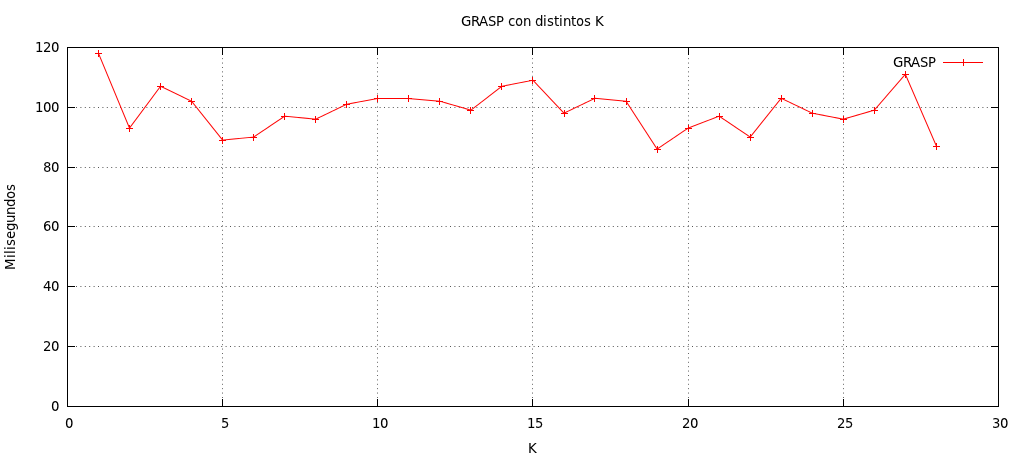
\includegraphics[width=15cm]{./graficos/GRASP_distintosK.png}
\end{center}

Como se puede notar en la imágen, el tiempo no varía ya que k se comporta como una constante al ser siempre menos a la cantidad de nodos, por lo que en caso de saber valores de la entrada en los que sabemos
que Greedy se comportaría mal al elegir siempre el mejor a partir de su estrategia, elegir un k más grande para poder elegir entre más nodos aleatoriamente, no arruina el tiempo de procesamiento.

Ahora se presenta un algoritmo con distintos grafos corrido cada uno con k = 5,10,15,20

\begin{center}
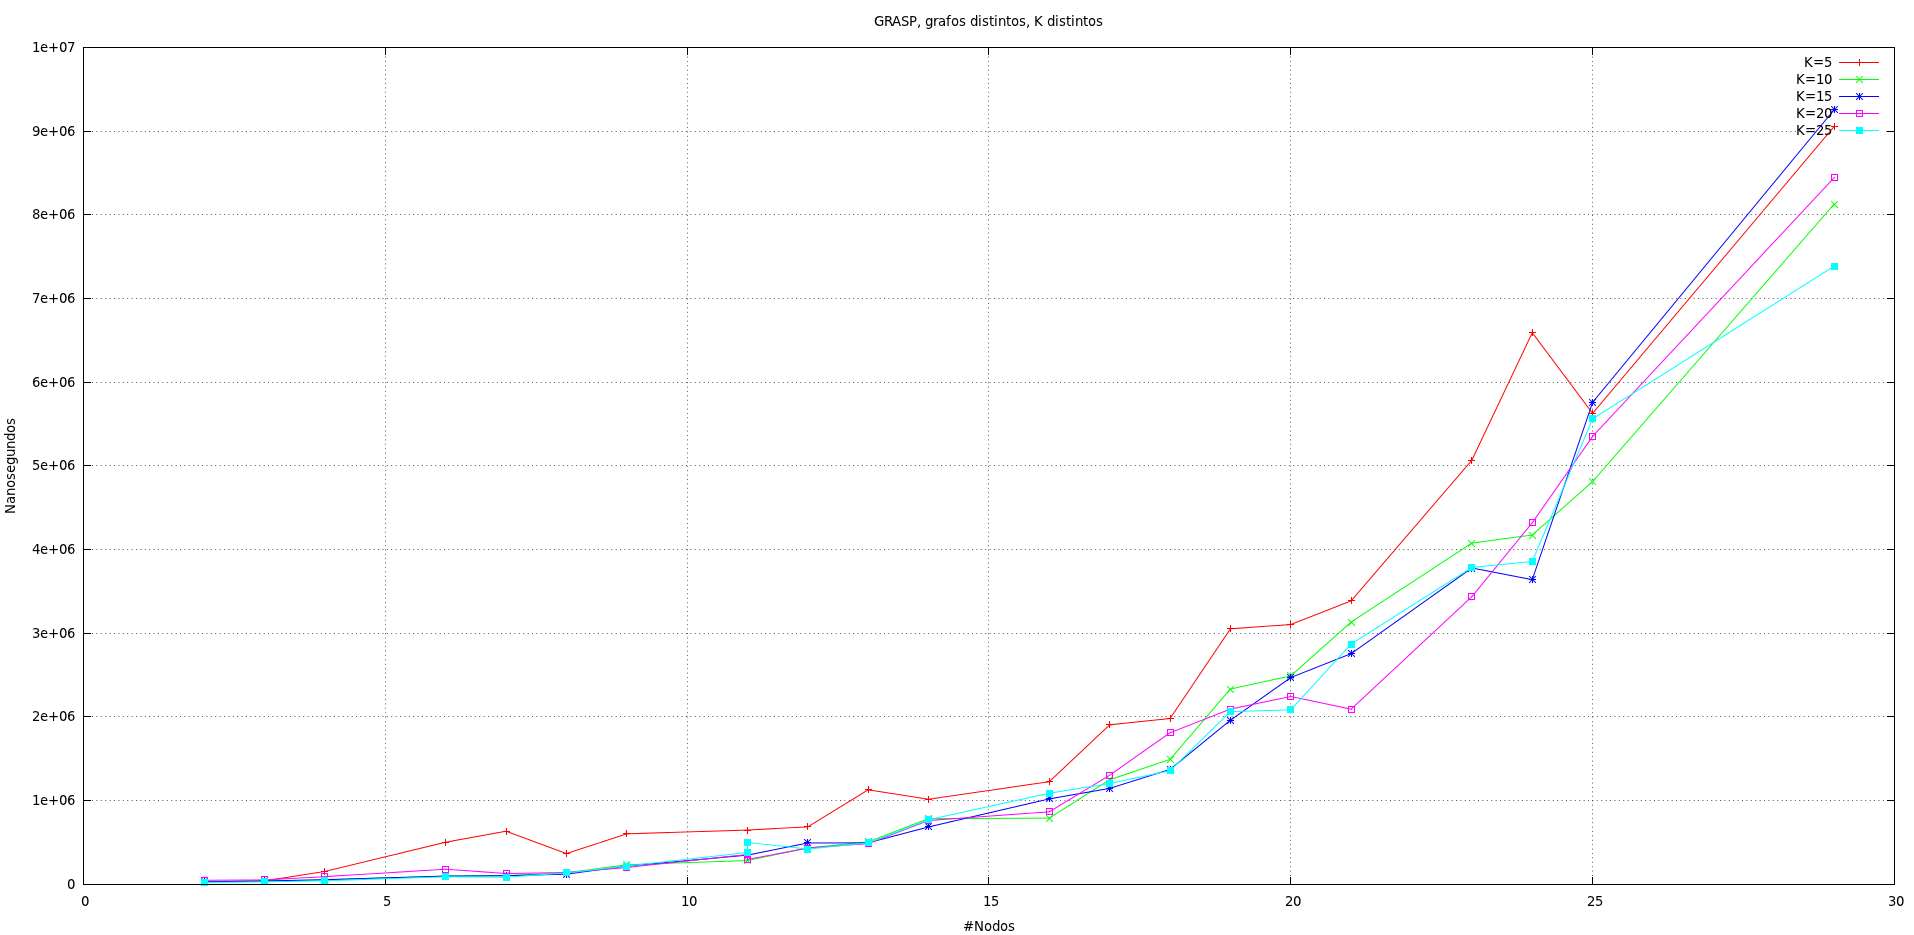
\includegraphics[width=15cm]{./graficos/GRASP_distGrafos_distK.png}
\end{center}

Tal como era esperado el algorimto hace menos operaciones cuando tiene menos nodos y el k multiplica el tiempo como una constante.
Sin embargo, es necesario tener en cuenta que, al depender de otros algoritmos como ser: Greedy y LocalSearch, que tienen una condición de corte distinta a la de este algoritmo, puede pasar que terminen antes o tarden más.
Es así que se explican la falta de paralelismo exacto de los gráficos. Por ejemplo, en caso de que greedy con un k, elija en tres iteraciones un conjunto dominante minimal y sin embargo para otro k elija en más iteraciones.

  \newpage
\section{Comparaciones}

\subsection{Introducción}

Realizamos diferentes gráficos generados pseudo-aleatoriamente con el fin de poder obtener una idea generalizada entre los algoritmos, ya que en las secciones anteriores pudimos
detallar los peores y mejores casos de cada uno. Estos algoritmos fueron generados con una función que recibe como parámetro la cantidad de nodos, y una probabilidad. Dicha función, por cada par de nodos, genera un valor random entre 0 y 1, si este valor está por debajo de la probabilidad recibida como parámetro, unirá dichos nodos, de otra manera, no.\\
Los análisis a realizar serán del estilo cantidad de nodos del conjunto dominante otorgado por cada heurística, comparándolo con el Exacto, y tiempos.\\
Para el GRASP, elegimos correr con k=15, ya que después de varias pruebas, nos pareció el que más se acercaba al óptimo antes de que el algoritmo entre en lo que denominamos "esperando mejor solución que puede no llegar" (remitirse al análisis del GRASP en la sección anterior).\\
Cabe destacar que el algoritmo exacto, se deja de correr para los n $>$ 30 debido a su complejidad.


\subsection{Exacto - Goloso}

Como vimos anteriormente el algoritmo Exacto tiene complejidad exponencial mientras que el Goloso polinomial. Es decir que para valores de entrada grandes el Goloso va a costar mucho menos ciclos. Por otra parte el Greedy puede devolver conjuntos dominantes no mínimos (es decir un conjunto dominante tal que exista un conjunto con menor cantidad de nodos que también sea dominante) mientras que el Exacto absolutamente siempre va a devolver el mínimo. \\
Teniendo en cuenta estos conceptos, para saber que algoritmo nos conviene usar tendríamos que tener en cuenta varias cosas. Si sabemos que las instancias de entrada rara vez serán con mas de un nodo del mismo grado, no nos afecta significativamente que el algoritmo nos devuelva esporádicamente resultados subóptimos y necesitamos que el algoritmo sea veloz, claramente la mejor opción es el Greedy. Ya que dificilmente fallaría (porque casi siempre vendrían grafos con todos nodos de distintos grados), funciona mucho más rápido que el exacto y el caso en que falle no sería decisivo. \\
Ejemplo:\\
Un ejemplo de la vida real de este caso podría ser si quisiese elegir a los referentes políticos de cada provincia de forma tal que representen a toda la población a través de la influencia en esta que ejercen . Donde influencia se entiende como gente que lo apoya y cada persona puede apoyar a mas de uno (esto se obtuvo a través de encuestas). El problema lo abstraeríamos a grafos diciendo que cada nodo es una persona y estas se relacionan si una apoya la otra (no importa quien a quien ya que entendemos que si un ciudadano apoya a un candidato político es porque este también apoyaría al ciudadano, un poco utópicos lo se). En este caso como por lo general los dirigentes políticos zonales tienen influencia gracias a los partidos políticos a los que pertencen y estos suelen diferir entre sí en la cantidad de adherentes (es muy raro que dos partidos tengan exactamente la misma cantidad de adherentes) entonces en la gran mayoría de los casos los grafos van a estar compuestos todos por nodos con distinto grado y además van a ser datos de entrada muy grandes (ya que cada provincia contiene como mínimo 100 mil habitantes) por lo tanto en este caso sería muchísimo mejor utilizar el Greedy. \\
En cambio si no me importa mucho el tiempo de proceso, se que los datos de entrada no van a ser muy grandes y necesito que el resultado sea siempre el mejor me conviene usar el exacto. Un caso de esto podría ser si mediante un mapa del circuito eléctrico de una ciudad del interior (es decir una ciudad chica) quiero obtener los puntos desde los cuales puedo llegar a todo el resto del tramado eléctrico para mejorar los transistores, para esto mediante la obtención del conjunto dominante mínimo obtendríamos estos puntos y los devolveríamos. Si consideramos que mejorar cada transistor nos cuesta cientos de miles de pesos es primordial que el resultado sea exacto y como solo deseamos correrlo una vez no es tan importante el tiempo que pueda tardar. Por eso en este caso la mejor opción sería el algoritmo exacto. \\

En el siguiente gráfico podemos apreciar la diferencia en ciclos entre estos algoritmos para distinta cantidad de nodos. Se puede ver claramente que a medida que el grafo tiene mas nodos la diferencia crece abisamalmente. Para el caso del exacto no pusimos los valores para todas las cantidades debido a que se hacía poco visible como evolucionaba la linea del goloso ya que el exacto alcanzaba valores muy muy grandes. 
\begin{center}
  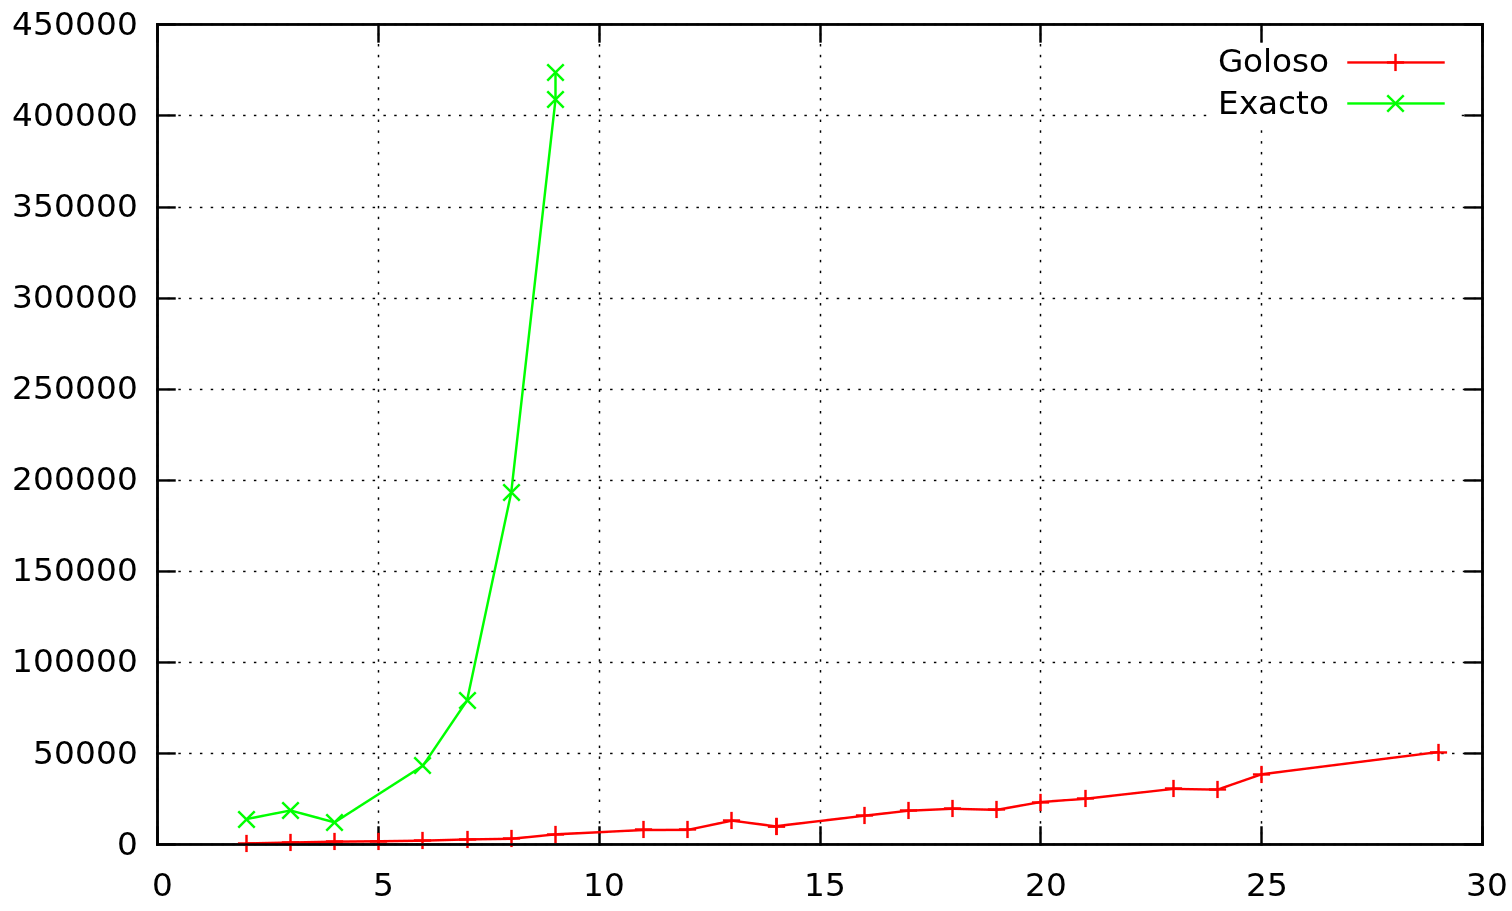
\includegraphics[width=12cm]{./graficos/comp_exacto_goloso.png}
\end{center}


\subsection{Exacto - Goloso - Local Search}
En ésta sección vamos a comparar tanto las soluciones obtenidas como el consumo de tiempo en éstos tres algoritmos. Decidimos hacerlo de ésta forma, y no separadamente, ya que el algoritmo greedy es parte (al menos, en nuestro caso), de la búsqueda local, y utilizamos el exacto para saber si las soluciones obtenidas son buenas o no. Por lo tanto, analizaremos los tres casos juntos. Para ello, vamos a ayudarnos de dos gráficos, donde podemos ver la cardinalidad de las soluciones para distinta cantidad de nodos, y el tiempo tomado para resolverlos. \\
\begin{center}
  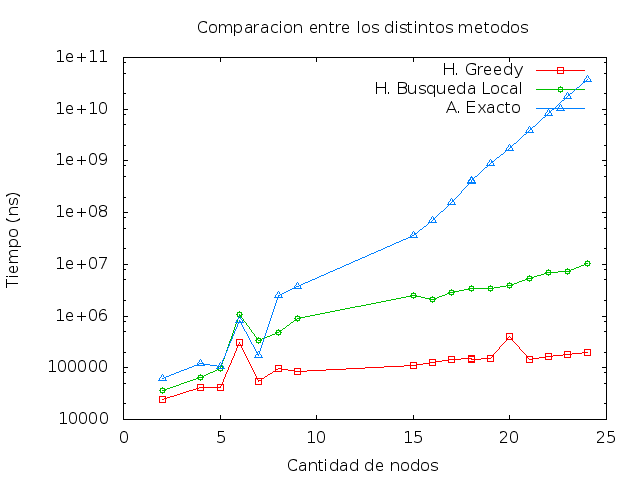
\includegraphics[width=12cm]{./graficos/local_comparacion.png}
\end{center}
Como vimos en el análisis anterior, para instancias muy pequeñas, y donde la exactitud es preponderante, el algoritmo exacto es el más adecuado a utilizar, ya que la diferencia de tiempo es muy poca, pero la diferencia de la solución podría ser considerable. En cambio, para entradas un poco más grandes (como podemos apreciar en el gráfico, de una diferencia de 5 nodos), ya no es conveniente utilizar el algoritmo exacto, ya que el tiempo que consume es exponencial a su cantidad de nodos, como podemos ver en el gráfico 1. En cambio, es recomendable utilizar alguno de los otros dos algoritmos que estamos analizando. \\
La gran diferencia entre el tiempo utilizado para encontra una solución con la búsqueda local y el algoritmo greedy, a pesar de tener complejidades parecidas, la podemos adjudicar a que en la búsqueda local, el proceso de encontrar soluciones "locales" se repite varias veces, y para varios métodos que tienen la misma complejidad (como ya dijimos antes, $n^2$), así que si bien consume más tiempo que la heurística golosa, ésta crece de forma polinomial, y es, por lejos, mucho mejor que la solución exacta, y muchas veces, como podremos analizar en párrafo y gráfico siguiente, nos ofrece una solución igual a la exacta o cuya cardinalidad difiere en 1 o 2 nodos únicamente. \\
Cuál de ellos es una pregunta que debe ser respondida según la situación y la exactitud de la solución que se busque, a partir del análisis de los gráficos 1 y 2 de ésta sección, donde se analiza la cantidad de soluciones y el tiempo demandado para encontrarlas. 

\begin{center}
  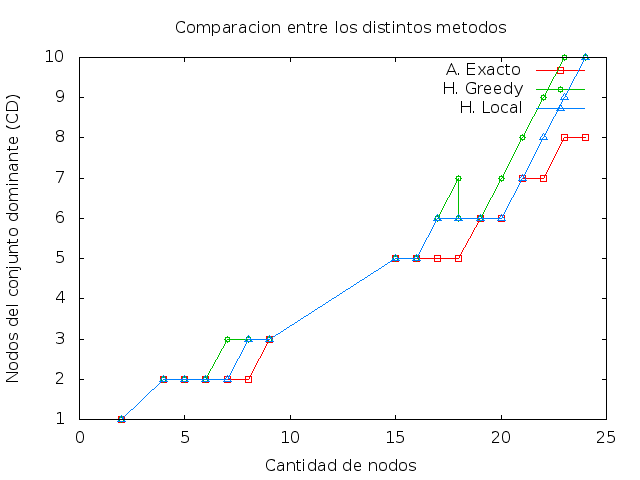
\includegraphics[width=12cm]{./graficos/local_comparacion_soluciones.png}
\end{center}

Por un lado, si sólo se desea encontrar un conjunto dominante, podemos utilizar la solución golosa, que es la más rápida de las 3 ya que no depende de ninguna otra solución. Por su parte, si la instancia es muy grande, pero deseamos que la solución sea lo más óptima posible, y que el tiempo de resolución sea polinomial, debemos utilizar la búsqueda local, ya que ha demostrado ser al menos tan mala como la solución greedy, aún en casos cuando la solución que le pasamos es el grafo entero (es decir, tomamos como conjunto dominante a todo el grafo, por más malo que eso sea). 


\subsection{Exacto - Goloso - Local Search - GRASP}

A continuación haremos una comparación masiva de los 3 primeros algoritmos contra GRASP.
Corremos distintos grafos con GRASP k=15, y los mismos grafos con los otros algoritmos.
\begin{center}
  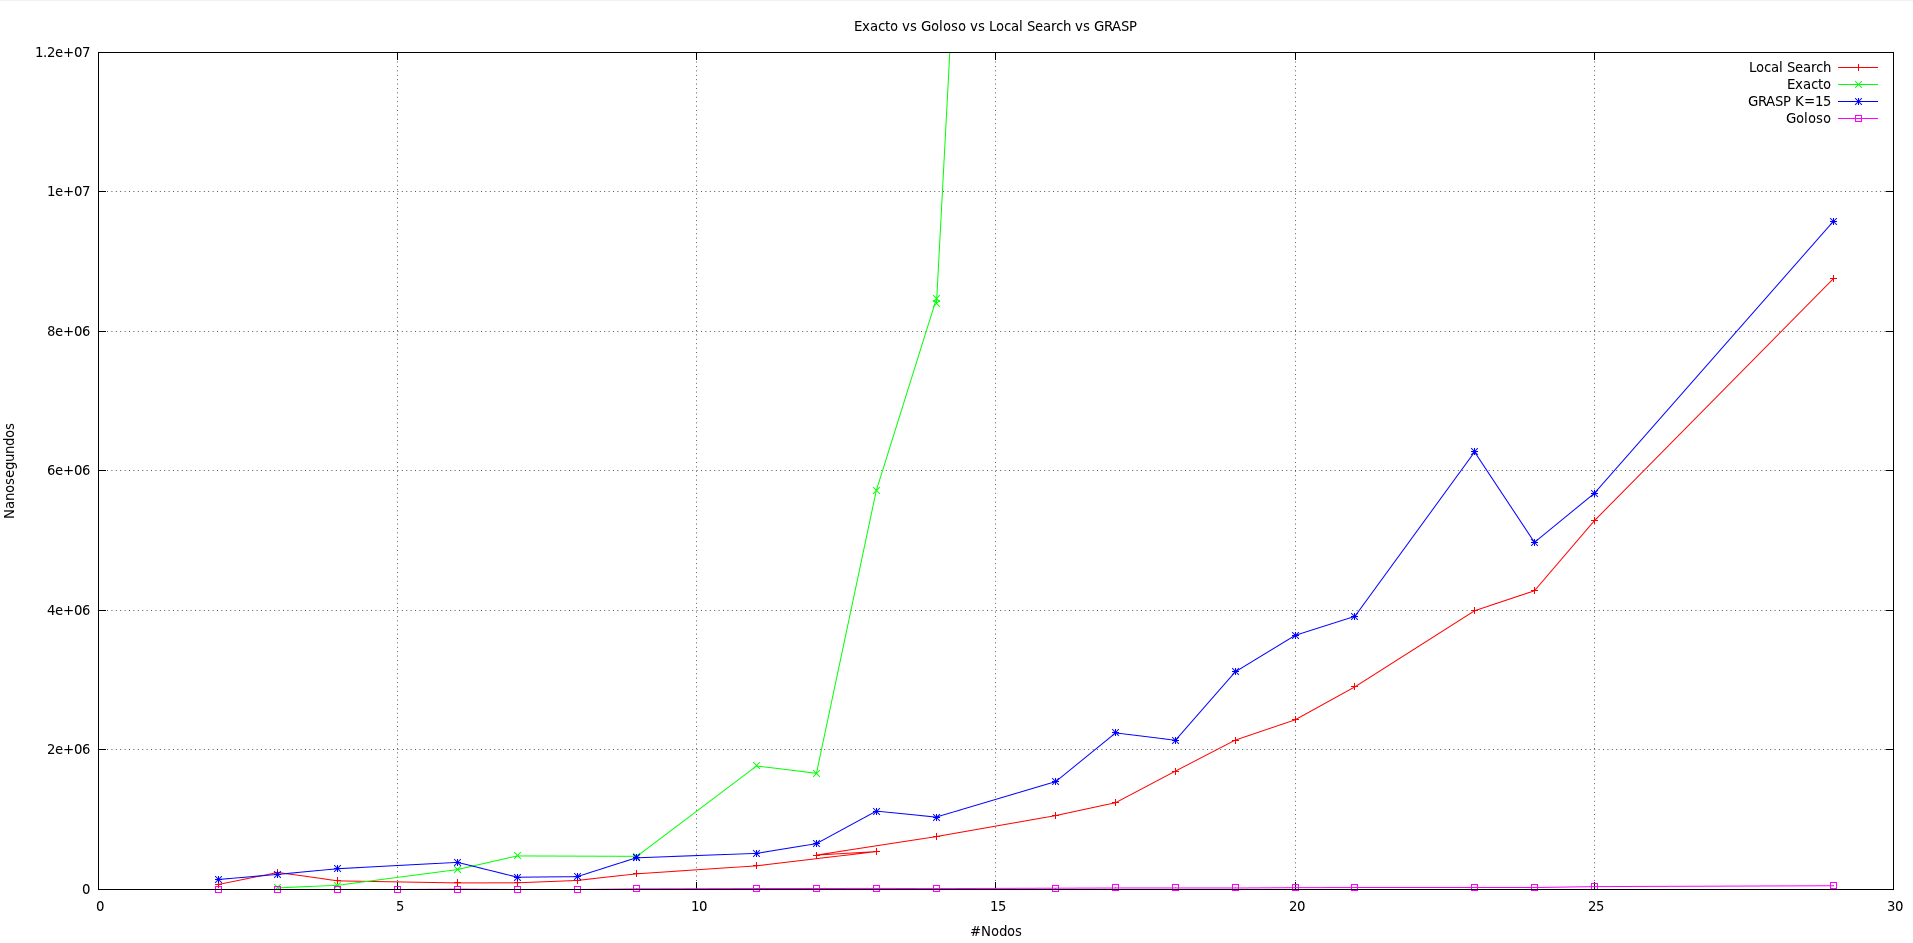
\includegraphics[width=15cm]{./graficos/todosVStodos.png}
\end{center}
Como vimos antes no hay una gran variación de tiempo de procesamiento más allá la diferencia entre la exponencialidad del Exacto contra la polinomialidad del resto, por lo tanto queremos aclarar que en caso de tener que resolver este
problema a través de una Heurística, fuertemente recomendamos ejecutar GRASP, ya que no existe gran diferencia de tiempos, y el algoritmo en el peor de los casos devuelve la misma cantidad de nodos que el goloso. Sin embargo, como ya 
mencionamos antes la cantidad de soluciones que puede devolver el GRASP se ve multiplicada por k, y a cada una de estas k soluciones se lo intenta mejorar localmente. Es por eso que, si sabés datos de la entrada 
del grafo en donde greedy pueda llegar a devolver un resultado lejos del exacto, es recomendable utilizar GRASP ya que aumentás las posibilidades y probabilísticamente podés conseguir una mejor solución.

  \newpage
\section{Apéndice}

$^{1}$http://docs.oracle.com/javase/6/docs/api/java/util/ArrayList.html

  \newpage

\end{document}
